%!TEX TS-program = xelatex
%!TEX encoding = UTF-8 Unicode

\documentclass[11pt,tikz,border=1]{standalone}
\usetikzlibrary{positioning}

\begin{document}
  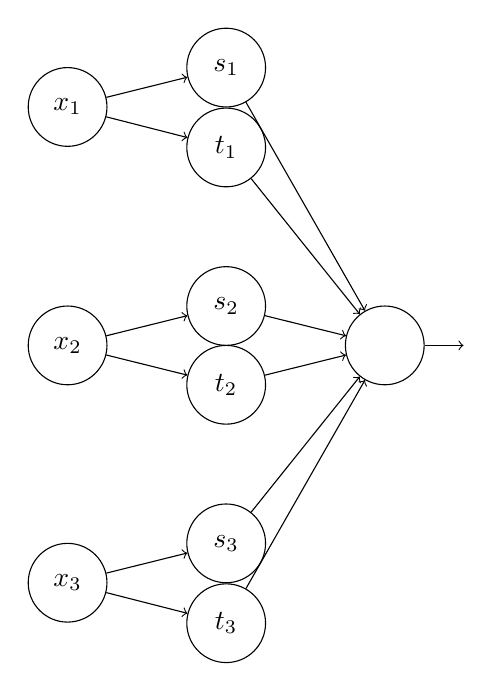
\begin{tikzpicture}[
    neuron/.style={circle,draw,inner sep=0pt,minimum size=10mm}
    ]
    
   \node(n) [neuron] {};
   
   \node(s2) [left=of n,neuron,yshift=5mm] {$s_2$};
   \node(t2) [left=of n,neuron,yshift=-5mm] {$t_2$};
    
   \node(t1) [above=of s2,circle,inner sep=0pt,minimum size=10mm] {};
   \node(s1) [above=of t1,neuron,yshift=-10mm] {$s_1$};

	\node(s3) [below=of t2,circle,inner sep=0pt,minimum size=10mm] {};
	\node(t3) [below=of s3,neuron,yshift=10mm] {$t_3$};    
    
    \node(x1) [left=of s1,neuron,yshift=-5mm] {$x_1$};
    \node(x2) [left=of s2,neuron,yshift=-5mm] {$x_2$};
    \node(x3) [left=of s3,neuron,yshift=-5mm] {$x_3$};
    
    \foreach \x in {1,2,3} {
    	\draw[->] (x\x) to (s\x);
    	\draw[->] (x\x) to (t\x);
    	\draw[->] (s\x) to (n);
    	\draw[->] (t\x) to (n);
    }
    
    \node(t1c) [neuron] at (t1.center) {$t_1$};
    \node(s3c) [neuron] at (s3.center) {$s_3$};
    
    \draw[->] (n) -- ++(10mm,0);
    
  \end{tikzpicture} 
\end{document}
